% last updated in April 2002 by Antje Endemann
% Based on CVPR 07 and LNCS, with modifications by DAF, AZ and elle, 2008 and AA, 2010, and CC, 2011; TT, 2014; AAS, 2016

\documentclass[runningheads]{llncs}
\usepackage{graphicx}
\usepackage{amsmath,amssymb} % define this before the line numbering.
\usepackage{ruler}
\usepackage{booktabs}
\usepackage[usenames, dvipsnames]{color}
\usepackage[width=122mm,left=12mm,paperwidth=146mm,height=193mm,top=12mm,paperheight=217mm]{geometry}
\usepackage{hyperref}

\usepackage{xspace}


\newcommand{\sz}[1]{\textcolor{blue}{\emph{//sz: #1//}}}
\newcommand{\cs}[1]{\textcolor{PineGreen}{\emph{//cs: #1//}}}
\newcommand{\la}[1]{\textcolor{cyan}{\emph{//la: #1//}}}

\newcommand{\vgenome}{VisualGenome\xspace}
\newcommand{\referit}{ReferIt\xspace}
\newcommand{\refcoco}{RefCOCO\xspace}
\newcommand{\refcocop}{RefCOCO+\xspace}
\newcommand{\flickr}{Flickr30k Entities\xspace}

\newcommand{\refexp}[1]{\textsl{#1}}
\newcommand{\word}[1]{\textsl{#1}}
\newcommand{\cat}[1]{\textsc{#1}}

\newcommand{\green}[1]{\textcolor{PineGreen}{#1}}
\newcommand{\red}[1]{\textcolor{red}{#1}}
\newcommand{\blue}[1]{\textcolor{blue}{#1}}
\newcommand{\yellow}[1]{\textcolor{yellow}{#1}}

\usepackage{pifont}
\newcommand{\cmark}{\ding{51}}%
\newcommand{\xmark}{\ding{55}}

\begin{document}
% \renewcommand\thelinenumber{\color[rgb]{0.2,0.5,0.8}\normalfont\sffamily\scriptsize\arabic{linenumber}\color[rgb]{0,0,0}}
% \renewcommand\makeLineNumber {\hss\thelinenumber\ \hspace{6mm} \rlap{\hskip\textwidth\ \hspace{6.5mm}\thelinenumber}}
% \linenumbers
\pagestyle{headings}
\mainmatter
\def\ECCV18SubNumber{***}  % Insert your submission number here

\title{Object naming is context dependent - A case study on testing linguistic hypotheses on real-world image corpora} % Replace with your title

\titlerunning{ECCV-18 submission ID \ECCV18SubNumber}

\authorrunning{ECCV-18 submission ID \ECCV18SubNumber}

\author{Anonymous ECCV submission}
\institute{Paper ID \ECCV18SubNumber}


\maketitle

\begin{abstract}
The abstract should summarize the contents of the paper. LNCS guidelines
indicate it should be at least 70 and at most 150 words. It should be set in 9-point
font size and should be inset 1.0~cm from the right and left margins.
\dots
\keywords{We would like to encourage you to list your keywords within
the abstract section}
\end{abstract}

@Carina TODO:
\begin{itemize}
	\item requirements: \\ 
	add most specific name; (possible ways to obtain information: taxonomy, object detectors) \\
	add unconstraint object co-occurrences / unbiased as far as possible; \\
	rename R1? (lexical alternatives? candidate names?)
	\item title?
\end{itemize}

\section{Introduction}

Understanding and modeling the way humans converse about their environment using natural language has been a long-standing goal of research in various fields related to artificial intelligence and linguistics.
With recent  developments in computer vision and a range of massive data collections in particular, there has been a veritable explosion of interest in language \& vision tasks, ranging from image captioning \cite{fangetal:2015,devlin:imcaqui,chen2015mind,vinyals:show,Bernardietal:automatic}, referring expression resolution and generation \cite{Kazemzadeh2014,mao15,Yu2016,schlazar:acl16}, to multi-modal summarization or visual dialogue \cite{das2017visual,vries2017guesswhat}.
In principle, the underlying data collections here should not only spur computational, application-oriented research aimed at implementing systems for very specific tasks -- they should also constitute extremely valuable resources for research aimed at deriving linguistic generalizations about various phenomena related to language grounding, reference and situated interaction which, for a long time, have been investigated mostly in very controlled and small-domain experimental settings, cf. \cite{anderson1991hcrc,fernangen:sigd07,krahmer:2012,takenobu2012rex,zarriess2016pentoref} for some examples of traditional data collections related to reference and grounding.  
In turn, these linguistic generalizations could inform computational modeling, architecture design and future data collections.
However, so far, studies that have tested linguistic hypotheses on large-scale vision \& language resources have been relatively rare. 


In this paper, we take a look at object naming, a core phenomenon that occurs in virtually every language \& vision task and is, at the same time, subject of ongoing research in language grounding and pragmatics. 
Our starting point is a particular linguistic hypothesis related to object naming - namely that the choice of a name for an object is dependent on other objects in its visual context - which has been tested recently in a classical experimental setting \cite{graf2016animal}. 
We discuss how this hypothesis could be tested based on recent data sets that pair images and object descriptions, referring expressions or captions (all containing object names) and define a set of requirements for obtaining a theoretically informed model for object naming.
In sum, this discussion will show that specific requirements are met by particular resources, but none of the available corpora consistently satisfies all of the requirements.
We believe that this is a perfect showcase illustrating the challenges for linguistically motivated research in language and vision, and we derive a proposal for obtaining more consistently designed and annotated data collections for object naming.


\section{Naming Objects (in Context)}
\label{sec:object_naming}

The act of naming an object amounts to that of picking out a nominal to be employed to refer to it (e.g., ``the \textit{dog}'', ``the white \textit{dog} to the left'').
Since an object is simultaneously a member of multiple categories (e.g., a young beagle is at once a dog, a beagle, an animal, a puppy etc.), all the various names that lexicalize these constitute a valid alternative, meaning that the same object can be named with more or less \textbf{specific names} \cite{brown1958shall,murphy2004big}. 
Seminal work on concepts by Rosch suggests that object names typically exhibit a preferred level of specificity called the \textbf{entry-level}. This typically corresponds to an intermediate level of specificity, i.e., \textbf{basic level} (e.g, \textit{bird}, \textit{car}) \cite{rosch1976basic}, as opposed to more generic (i.e., \textbf{super-level}; e.g., \textit{animal}, \textit{vehicle}) or specific categories (i.e., \textbf{sub-level}; e.g., \textit{sparrow}, \textit{convertible}). However, less prototypical members of basic-level categories tend to be instead identified with sub-level categories (e.g., a penguin is typically called a \textit{penguin} and not a \textit{bird}) \cite{jolicoeur1984pictures}. This out-of-context preference towards a certain taxonomic level is often referred to as \textbf{lexical availability}. 

While the traditional notion of entry-level categories suggests that objects tend to be named by a \textit{single} preferred concept, research on pragmatics has found that speakers are flexible with respect to the chose level of specificity.
Scenarios where multiple objects (of the same category) are present induce a pressure for generating names which uniquely identify the target \cite{olson1970language}, such that sub-level names can be systematically elicited in these cases \cite{rohde2012communicating} \cite{graf2016animal}. For example, in presence of more than one dog, the name \textit{dog} is ambiguous and a sub-level category (e.g., \textit{rottweiler}, \textit{beagle}) is more informative and potentially preferred by speakers, though additional factors such as cost (which is typically approximated by frequency) or saliency also come into play \cite{graf2016animal}  \cite{clark1983common}.
%Note that reasoning about the informativeness of a name require categorization of all the potential referents in that context (e.g., to know that \textit{dog} is ambiguous require having recognized that there are multiple dogs in the scene). 
%Other contextual factors affecting lexical choice include the \textbf{perceptual salience} of the object, such as its size or location \cite{clark1983common}.

So far, research in computer vision, and vision \& language, has mostly worked around the fact that objects can be categorized and named at different levels of specificity.
 State-of-the-art object recognizers are typically trained on a flat set of categories taken from ImageNet (REF!!), though see work by Deng et al. on trading off object recognition accuracy and level of specificity \cite{deng2012hedging}.
\cite{Ordonez:2016} present one of the few explicit studies on naming in computer vision and operationalize the task as translating between leaf nodes in the ImageNet hierarchy and entry-level
 concepts, adopting the traditional view that there is a single preferred name for a given object.
 Thus, establishing whether object naming is context dependent in realistic, large-scale data sets would not only be of interest to theoretical work on concepts and pragmatics, it would also be of great importance for the design of models in computer vision, object recognition and vision \& language.

\section{Requirements}
\label{sec:requirements}

\begin{figure}[t]
	\begin{center}
		\begin{minipage}{.52\textwidth}
			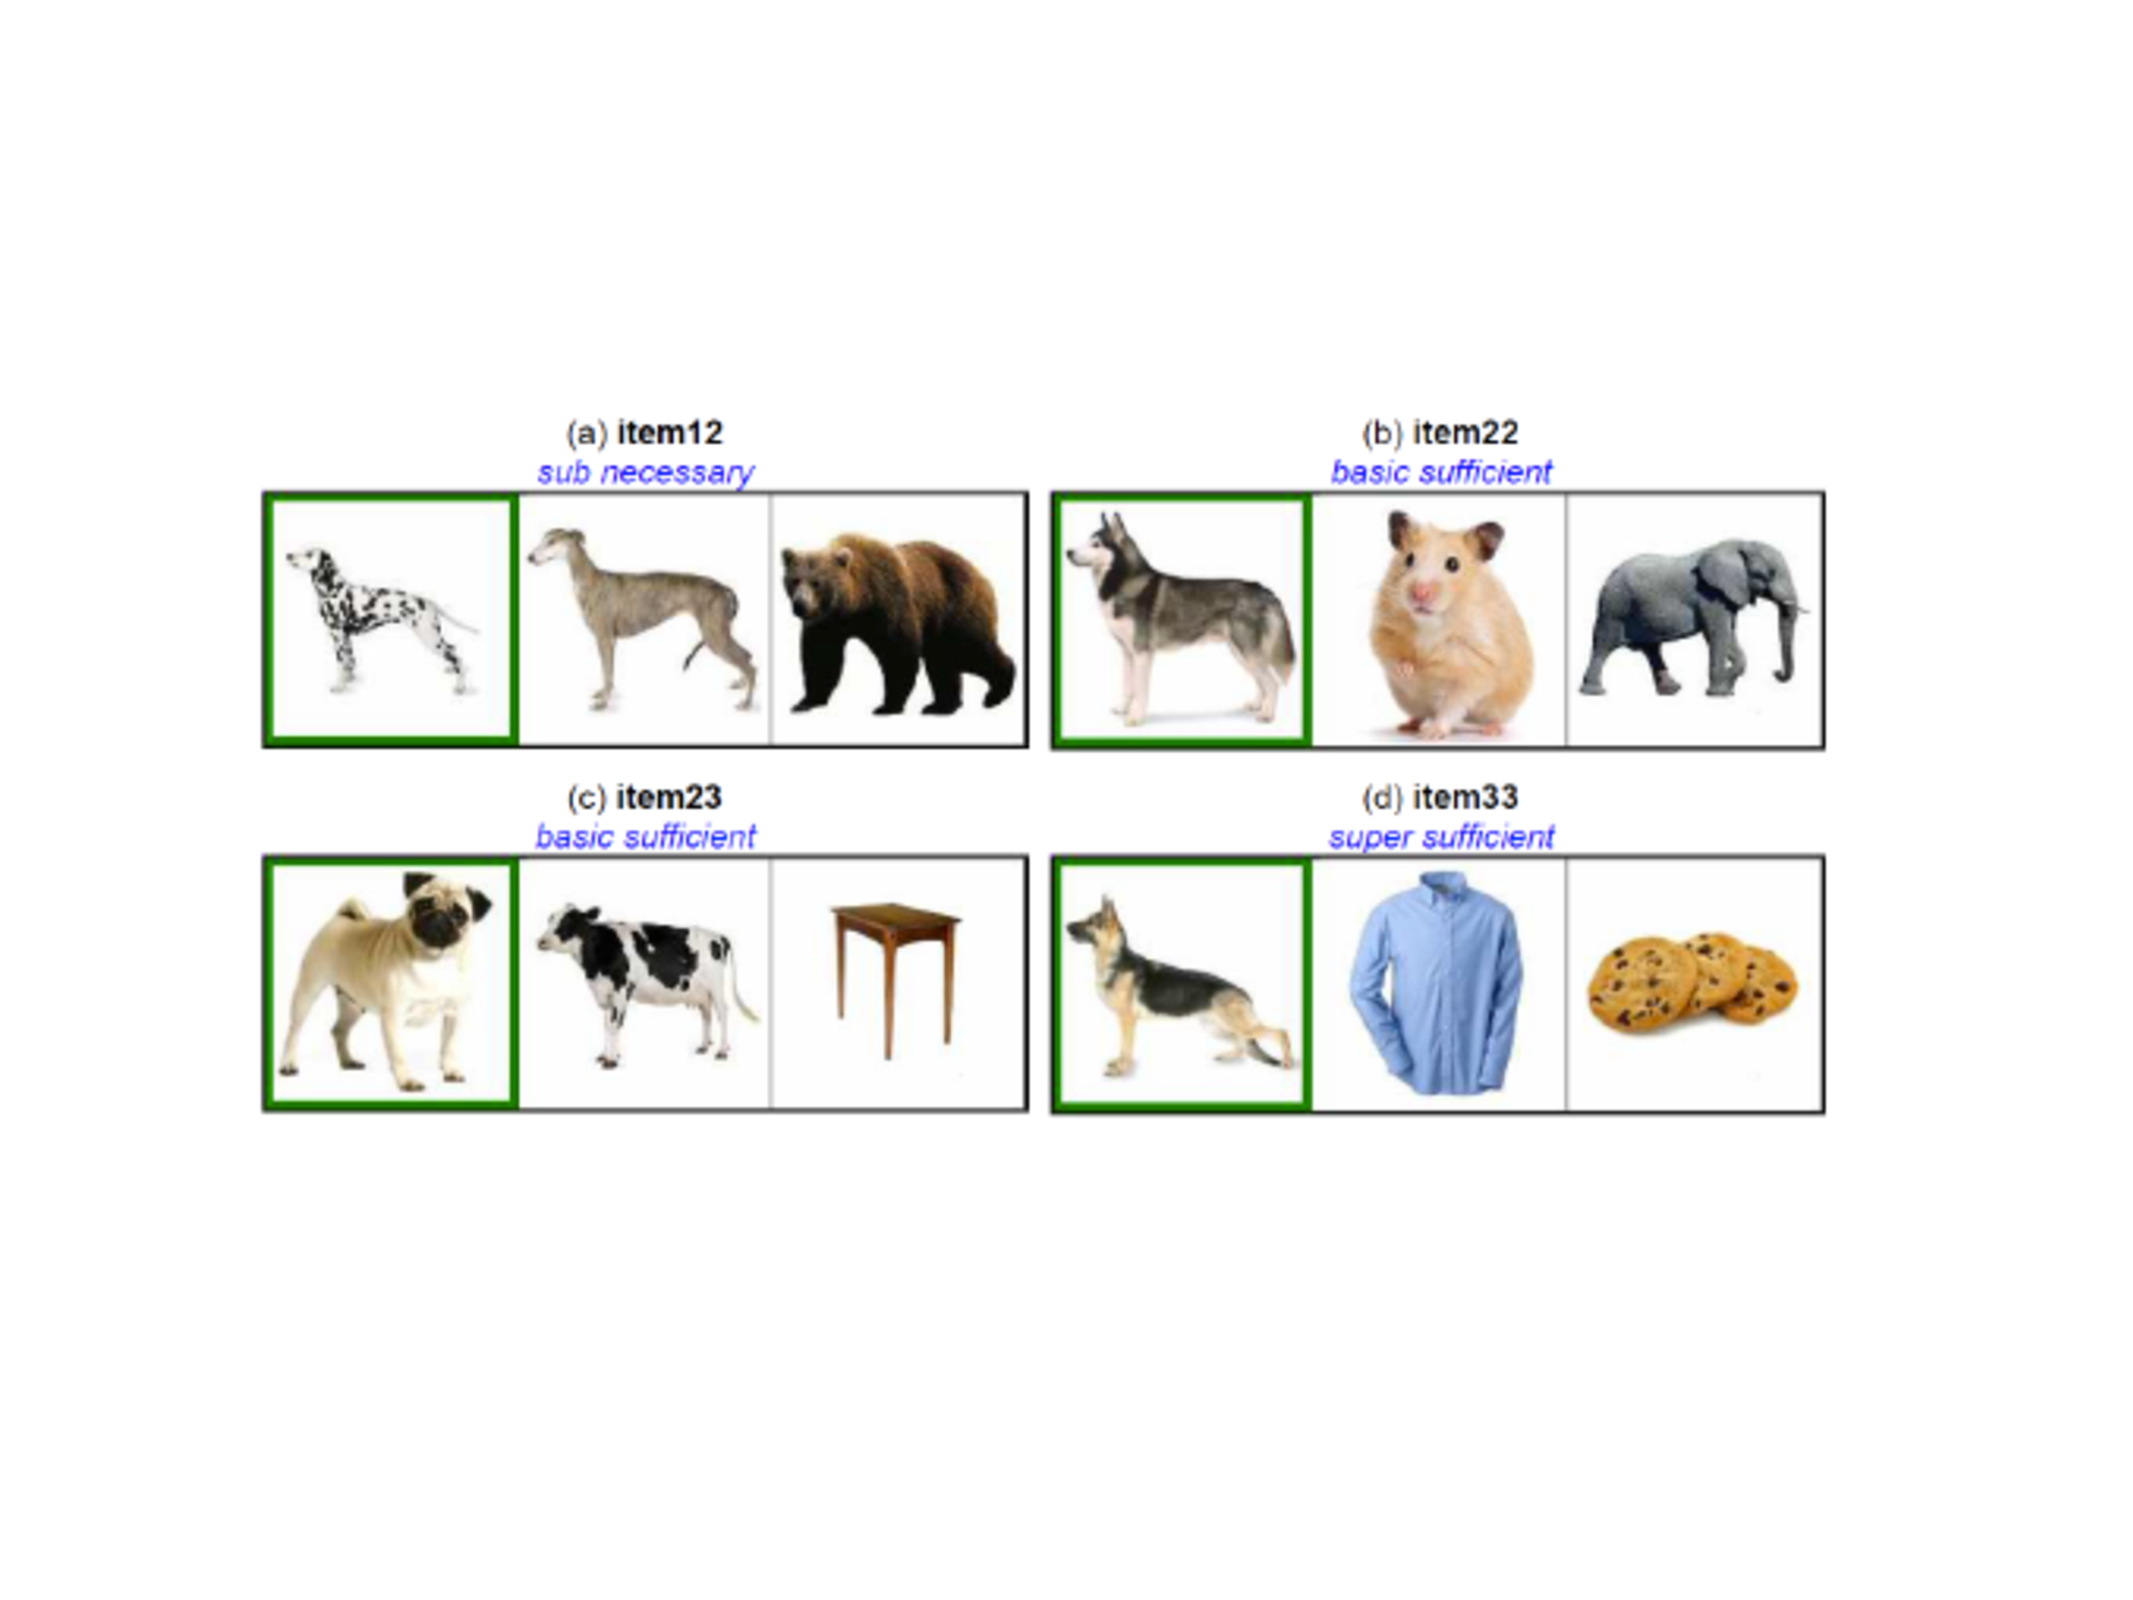
\includegraphics[width=\linewidth]{fig/graffig.pdf}
		\end{minipage}
		\begin{minipage}{.42\textwidth}
			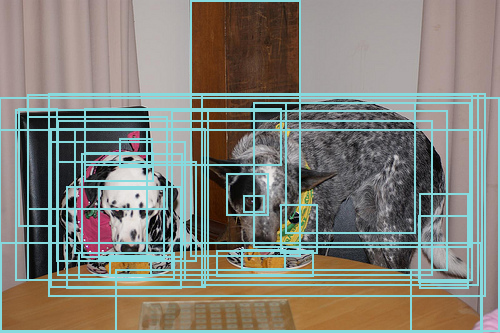
\includegraphics[width=5cm]{fig/visual_genome_dogs.png}
		\end{minipage}
	\end{center}
	\caption{Experimental and real-world visual scenes showing dogs (GET MORE IMAGES OF DOGS FROM VG???)}
	\label{fig:graf_genome}
\end{figure}

In this Section we discuss requirements for scaling experimental studies on object names as in \cite{graf2016animal} to real-world images.
The difference between these two approaches is illustrated in Figure \ref{fig:graf_genome}, showing  \cite{graf2016animal}'s carefully controlled experimental conditions with isolated objects arranged in a collage, and a real-world scene where multiple objects occur in a natural context.
Thus, in contrast to \cite{graf2016animal} we do not aim for assembling controlled and, to some extent, artificial scenes, but we aim for studying object naming as prompted by real-world images. Therefore, we not only need access to names naturally generated by speakers, but also, we need to be able to quantify those factors whose interaction with naming we want to analyze. 

Given a natural scene with multiple objects and a target object that a speaker referred to, we need to be able to answer the following questions:

\begin{itemize}
        \item[(1)] \textbf{Lexical choice}: \\
        Which name did the speaker use to refer to the target object?
		\item[(2)] \textbf{Lexical candidates}: \cs{"candidate" does not exclude the chosen name in contrast to "alternative"}\\
		%Which names are available for the target objects?  
		Which names are available for the target objects? 
		And how are they taxonomically related? 
		For instance, if we want to check whether a convertible is more often referred to with a basic-level category (e.g.,~\refexp{car}) or a more specific one (e.g.,~\refexp{convertible}) we need to know that a given object is a \cat{convertible}, and that \cat{convertible} is a sub-level concept of \cat{car} (and \cat{vehicle}, etc.). 
		%Additionally, in
		In \cite{graf2016animal}, the authors manually group object names used by speakers in terms of three levels (sub-level, basic-level, super-level). 
		Thus, ideally, %names 
		lexical candidates 
		would be grouped according to their taxonomic relations. 
		\item[(3)] \textbf{Contextual informativeness}: \\
		Which names are available for the other objects in the scene (i.e. distractors)?
		For instance, when the target is a \cat{convertible}, we need to know that there are multiple \cat{convertibles}, \cat{cars}, etc. to judge whether these concepts are ambiguous.
\end{itemize}

\cs{Should the following be here or at the beginning of Sect. 4?}
\cs{We could also call below requirements "Desiderata"}
In practical terms, the prerequisite for Requirements~(2) and~(3) is, given an image, the information on \textbf{R1: the most specific category} of \textbf{each object} which is depicted in the image. 
A taxonomy, such as WordNet \cite{fellbaum1998wordnet}, could then be queried with these categories to retrieve their individual lexical candidates arranged by their taxonomic relations. \\
Furthermore, the information on the \textbf{R2: entry-level category} of an object could be used as a pivot to taxonomically group its lexical candidates.  

With respect to linguistic data-driven experiments, the range of linguistic phenomena under study (see, e.g.,~Section~\ref{sec:object_naming} for phenomena in object naming) need to be observable in the data in order to study the interaction of their underlying factors. 
Hence, a further practical requirement is that the data, first, captures ideally all possible combinations of the factor values across all factors\footnote{For example, data that contains only images where target and distractor objects do not share any lexical candidates would not be appropriate}, and second, that it has been naturally produced in that speakers were not constraint in their choice of a name by external factors. 
We summarize this requirement by the term \textbf{R3: unconstraint}. 
Note that this requirement XXX \cs{@Sina ref to bias and paper you mentioned?}.

\section{Resources: What Do We Have?}
\label{sec:resources}
%\begin{table*}[t]
	\begin{tabular}{|l||l|c|c|c|c|c|c|}
		\hline
		Resource
		& Purpose 	& \#Cat & \#Ref/ & \#Refs
		& \multicolumn{2}{c|}{Constraints on} 
		& WordNet  \\
		& & & object			
		& 			
		& language 	& images 
		& IDs?\\
		\hline \hline
		\refcoco 	& REG,REC
					& 80 & 3 & 50k
					& -				
					& $\geq$2 objs  
					& \xmark \\
					&
					& & & 
					& 
					& of same cat
					& \\
		\refcocop 	& REG,REC
					& 80 & 3 & 50k
					& + 			
					& $\geq$2 objs  
					& \xmark \\	
					&
					& & & 
					& 
					& of same cat
					& \\
		\flickr 	& Phrase localization
					& ?	& & 
					& -- 
					& & \xmark \\
					& Caption generation
					& & & &  \\
		\vgenome 	& Scene understanding 
					& 80k & & 
					& & & \cmark\\
					& Phrase localization
					& & & &  \\
		\hline
	\end{tabular}
	\caption{\label{tab:summary_resources} Overview of V\&L benchmarks for taks related to reference. Cat: Categories; Ref: Reference; REG and REC: Referring expression generation and comprehension, respectively.}
\end{table*}

\begin{table*}[t]
	\begin{center}
	\begin{tabular}{|l|c|c|c|c|}
		\hline
		Resource & \multicolumn{3}{c|}{Provides (more or less directly)}\\
		 		 & R1: Root-level & R2: Entry-level & R4: Coordinates  \\
		\hline \hline
		\refcoco 	& \xmark & \xmark & \cmark \\
		\refcocop 	& \xmark & \xmark & \cmark \\
		\flickr 	& \xmark & (\cmark) & \cmark \\
		\vgenome 	& \xmark & \cmark 	& \cmark \\
		\hline 		
	\end{tabular}
	\caption{\label{tab:summary_resources} BLABLA overview of resources and their shortcomings wrt object naming. REG and REC: Referring expression generation and comprehension, respectively.}
	\end{center}
\end{table*}

\subsection{Linguistic Resources, Computer Vision Resources}
\paragraph{WordNet}
WordNet \cite{fellbaum1998wordnet} blabla. 

\paragraph{Methods: Object Detectors, Image Classifiers} \cs{Do we need that? I would say no.}

\paragraph{ImageNet and ILSVRC}


\paragraph{MS COCO} \cite{mscoco}
MS COCO is an object recognition dataset of images of natural scenes of $91$~common object categories (e.g.,~\cat{dog, pizza, chair}). 
Multiple datasets for vision \& language tasks have been built on top of COCO, such as the referring expressions datasets \refcoco and \refcocop which we will discuss below, and \textsl{COCO Captions} \cite{chen2015cococaptions}.  
The latter provides five captions for each of  $300k$~images, spanning $80$~of the COCO categories.  
However, the COCO region-level (object) annotations are not linked to the captions.
\subsection{V\ \&\ L Resources}

\paragraph{\refcoco and \refcocop \cite{Yu2016}}~\\ 
Both datasets are extensions of \referit\cite{Kazemzadeh2014}, a large-scale collection of referring expressions (RE) for natural objects in real-world images, and are built on top of the MS COCO image collection \cite{mscoco}. 

The REs were collected via crowdsourcing in a two-player game, which was designed to obtain REs uniquely referring to the target objects in an image. 
Specifically, a director and a matcher are presented with an image, and the director produces a RE for an outlined target object in the image. 
The matcher must click on the object he thinks the RE refers to. 
If the matcher's prediction is correct, the RE is considered valid. 
For more details on the datasets see \cite{Yu2016}.

Finally, \referit is based on the SAIAPR image collection \cite{Grubinger2006} (20k images;99.5k image regions;120K REs), and captures not only REs for objects ("things") but also for scene categories (e.g.,{\refexp{grass, road}) (see also \cite{hu2015,mao2016generation}). 
The task of scene detection is beyond the focus of our study regarding object naming, we therefore will not discuss this dataset further.

\paragraph{Flickr30k Entities}~\\
The \flickr dataset \cite{plummer2015flickr30kentities}\footnote{Available at  \url{web.engr.illinois.edu/~bplumme2/Flickr30kEntities}}  augments Flickr30k, a dataset of 30k~images and five sentence-level captions for each of the images, with region-level annotations. 
Specifically, mentions of the same entities across the five captions of an image are linked to the bounding boxes of the objects they refer to. 
The dataset was designed to advance image description generation and phrase localization in particular (e.g.,~\cite{rohrbach2016grounding,plummer2017phrase,yeh2018unsupervised}). 
% 276k~manually annotated bounding boxes (i.e.,~entities are grounded in the image).
%
%
% augments the 158k captions from Flickr30k with 244k coreference chains, linking mentions of the same entities across different captions for the same image, and associating them with 276k manually annotated bounding boxes. Such annotations are essential for continued progress in automatic image description and grounded language understanding. They enable us to define a new benchmark for localization of textual entity mentions in an image.

\paragraph{\vgenome}~\\
\vgenome \cite{krishna2016visualgenome} aims to provide a full set of descriptions of the scenes which images depict in order to spur complete scene understanding. 
It contains a dense region-based labeling of $108k$~images with textual expression of the attributes and references of objects, their relationships as well as question answer pairs, all linked to WordNet synsets \cite[see below]{fellbaum1998wordnet}. 

\iffalse 
5.4 Million Region Descriptions
1.7 Million Visual Question Answers
3.8 Million Object Instances
2.8 Million Attributes
2.3 Million Relationships
Everything Mapped to Wordnet Synsets
\fi

\subsection{Discussion of Shortcomings}
We discuss the shortcomings of the presented V\&L datasets with respect to their use for computational linguistic studies of reference in general, and in particular in how far they satisfy the requirements for the study of object naming which we put forward in  Section~\ref{sec:requirements}. 

\paragraph{\refcoco and \refcocop}
The REs for both, \refcoco and \refcocop, were collected under the constraints that (i) all images contain at least two objects of the same category (80 COCO categories), which prompts the players to avoid the mere object category as RE, and (ii) in \refcocop the players must not use location words, urging them to refer to the appearance of objects. \cs{Maybe people tended more to use REs expressing the function of the object?}
%
While these constraints ensured that the datasets are interesting from the computer vision perspective, they fall short in containing phenomena that are intriguing from the view of language research: 
%
The range of linguistic phenomena under study (see, e.g.,~Section~\ref{sec:object_naming} for phenomena in object naming) need to be observable in the experimental data in order to study the interaction of their underlying factors. 
This is not given in \refcoco(+) with respect to the study of reference. 
First, how the choice of a RE for an object interacts with the categories of its distractors can only partially be observed in the data\footnote{For example, the preference of the entry-level category over a sufficiently unique more generic category can only be observed in images in which the target and the distractor objects are of different more generic categories.} due to~(i). 
And second, the study of how people \textit{naturally} refer to objects requires that speakers are not constraint in their choice of REs, which (ii)~does not fulfill.

Another critical property of the data is that, (iii), not all objects in an image were annotated with REs, may it due to the frequency constraint~(i), or due to the object not being part of the 80 COCO categories. 

%(i) violates (R0: The data contains only examples of case11, and excludes examples of case22, case23, case33 (case33:) do humans choose a basic-level category (e.g.,~\refexp{dog}) even though the super-level (e.g.,~\refexp{animal}) would suffice to uniquely refer to the object?). 

% the cost of a name and the contextual ambiguity it creates (see Section~\ref{sec:object_naming}), 
% entry-level category 

With respect to the problem of object naming, \refcoco(+) does not fulfill requirement~R1. 
As explained in Section~\ref{sec:requirements}, we can retrieve less specific categories from a taxonomy, but the most specific category of \textit{each} object depicted in an image needs to be provided by the data. 
This is not the case due to property~(iii), as well as due to the fact that the $80$~COCO categories tend to be entry-level categories. \cs{TODO: EX / ANALYSIS}
%
%However, the leaf category cannot be retrieved, disallowing us to determine whether target and distractors are of the same most specific category. 

The dataset also falls short in fully meeting requirement~R2 due to property~(iii)---it only covers 80~object categories---and constraint~(i) to some extent---we may not be able to reliably infer the basic-level from the data \cs{TODO: Example or remove last part}. 

\paragraph{Solution to R2: Captions?}
Additional REs could be collected from the COCO Captions dataset. %, which provides 5 natural language descriptions for each image in MS COCO. 
Since annotators could naturally refer to depicted objects in their descriptions (i.e.,~choose the entry-level as the most preferred reference whenever possible), we may infer the entry-level of the objects from them through maximum likelihood estimation. 
%
In contrast to \flickr, though, the data does not contain region-phrase associations,  % (i.e.,~object mentions are not linked to the corresponding image regions). 
such that natural language phrases first needed to be aligned with the image regions they refer to. 
This task of \textit{language grounding}, which has been an active research topic in vision \& language (e.g.,~\cite{kong2014what,karpathy2015deep,rohrbach2016grounding}), is beyond the focus of our object naming study. 
% We could also examine the bias shift of speakers (e.g.,~sparrow vs. bird may depend on the person)

\paragraph{Solution to R1: Object detectors?}
An alternative would be to apply object detectors or image classifiers trained to predict the most specific category of the full inventory of objects which the dataset covers. 
However, pre-trained models only exist for a subset of the datasets' objects. \cs{TODO: ADD CMP WITH ILSVRC}
For the training of a model using, e.g., ImageNet \cite{imagenet_cvpr09}, on the other hand, the  set of sub-level categories covered by the data need to be provided or collected from humans. 

\paragraph{\flickr}
By design, \flickr can be used to study the way people refer to individual entities in an image in dependence on the situation the speakers describe. 
In contrast to \refcoco(+), the production of entity mentions did not underlie any constraints. 
We can therefore gather naturally produced object names from the data and may be able to infer their entry-level categories. 
%
This is only the case for objects which are mentioned in the captions, which is why \flickr does not fully satisfy requirement~R2 \cs{ADD EXAMPLE IMAGE}. 

\flickr does not meet requirement R1 for similar reasons as \refcoco(+). 
Object categories tend to be even less specific than those of COCO (e.g.,~\cat{people, animals, bodyparts, clothing}), or are abstract (\cat{other, scene}).

Note that \flickr is less suited for referring expression generation and interpretation\cs{use the term grounding, interpretation or understanding to refer to the process of linking language to an image region?}, though, in that the mentions in isolation of their linguistic context may not uniquely identify the referred object. 
For example, the two men shown in the image in Figure~\ref{fig:ex_flickr} are  referred to by \refexp{a man} or \refexp{a guy}.

\begin{figure}[t]
	\begin{center}
		\begin{minipage}{.32\textwidth}
			%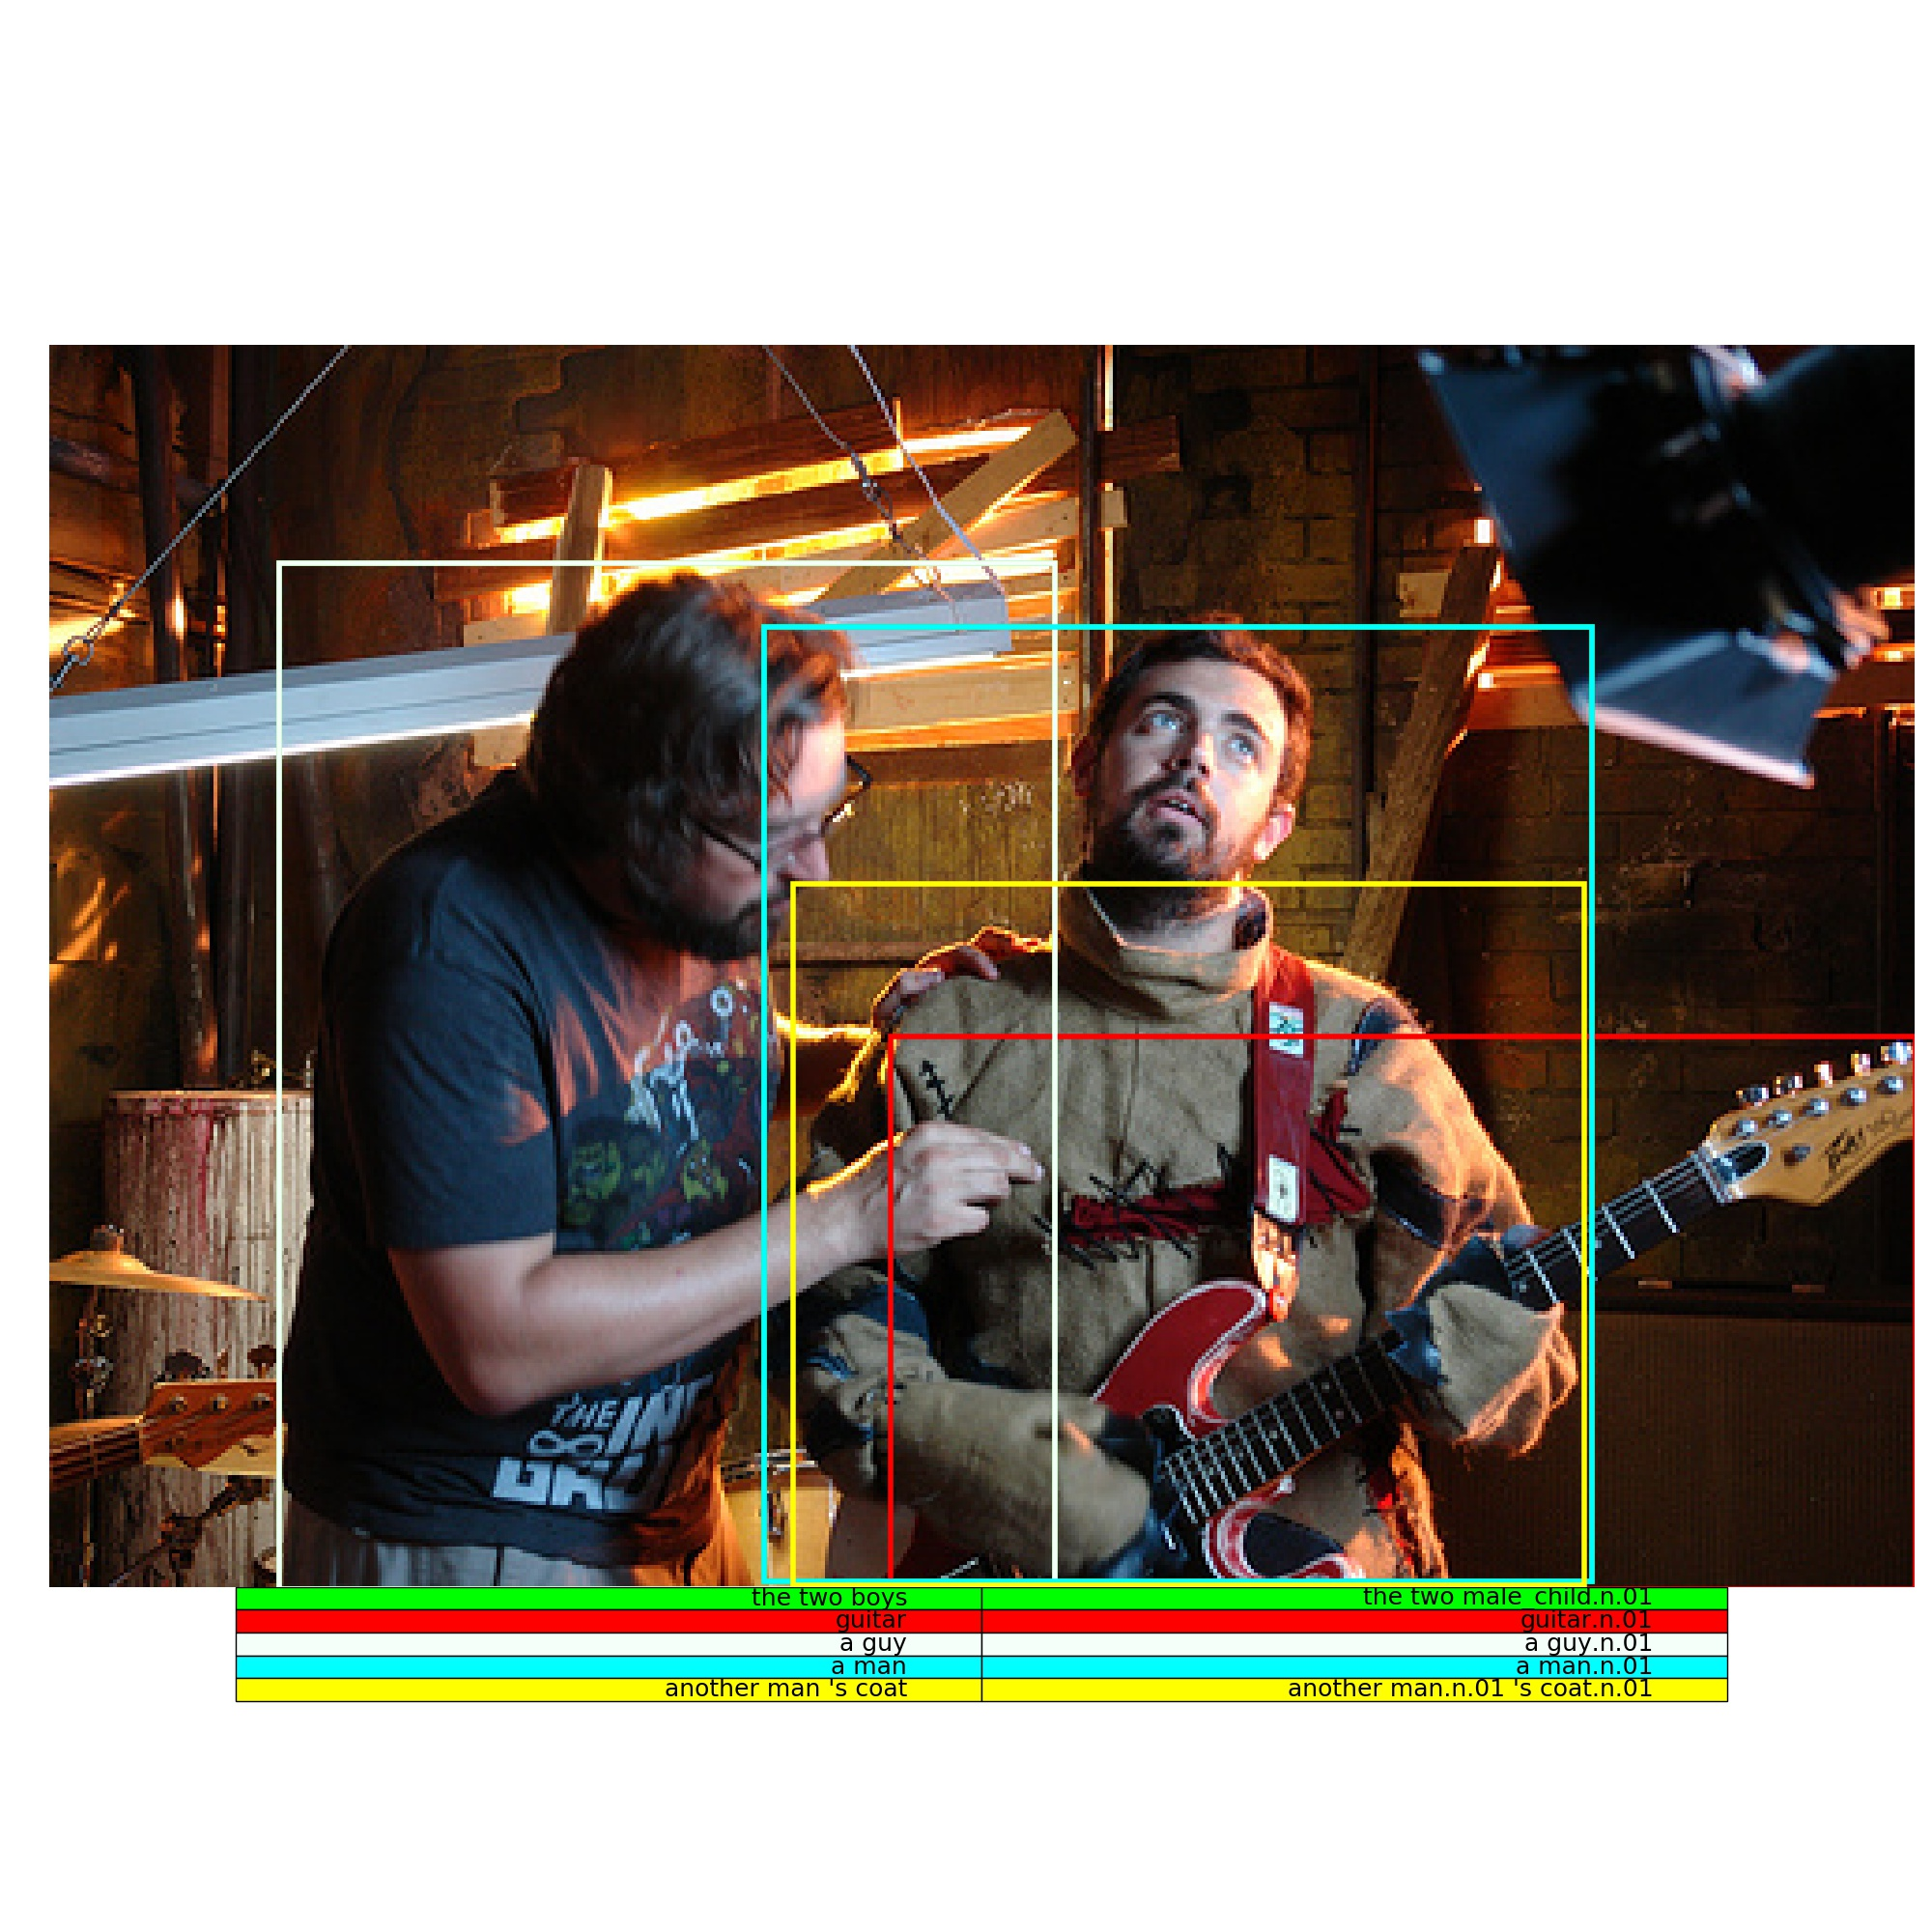
\includegraphics[width=4cm]{fig/flickr_1000523639_boxes.jpg}
		\end{minipage}
		\begin{minipage}{.67\textwidth}	
				{
			\begin{tabular}{l}
				\hline
				\green{[EN$_{39}$ Two people]} in {[EN$_{45}$ the photo]} are playing\\
				\; \red{[EN$_{40}$ the guitar]} and {[EN$_{41}$ the other]} is poking at {[EN$_{0}$ him]} .\\
				
			\blue{[EN$_{42}$ A man]} in \yellow{[EN$_{43}$ green]} holds \red{[EN$_{40}$ a guitar]} while \\
			\;{[EN$_{41}$ the other man]} observes \yellow{[EN$_{43}$ his shirt]} .\\
		
		{[EN$_{41}$ A man]} is fixing \yellow{[EN$_{43}$ the guitar players costume]} .\\
	
	{[EN$_{41}$ a guy]} stitching up \yellow{[EN$_{43}$ another man 's coat]} .\\
	
	\green{[EN$_{39}$ the two boys]} playing \red{[EN$_{40}$ guitar]} \\
	\hline
			\end{tabular}
			}
		\end{minipage}
	
		\caption{Example of \flickr. \label{fig:ex_flickr}}
	\end{center}
\end{figure}



\paragraph{\vgenome}
From a linguistic perspective, object categories (e.g.,~\cat{fawn}, \cat{industrial park}, \cat{opened bag}, \cat{carpet oriental}) are defined pragmatically, and the annotations are rather unstructured. 
For example, as illustrated in Figure~\ref{fig:ex_visualgenome}, the categorization of expressions into one of the three annotation types (region, attributes and relationships), is based on the verbs (\word{is} denotes attributes) and prepositions (\word{at} or \word{in} denotes relationships) \cs{double-check w/ paper}
Note also the spelling mistakes (e.g.,~\word{dalmation}, \word{wating}). 
Furthermore, regions and their annotations are highly redundant in that expressions referring to the same object may still be linked to different bounding boxes\cs{We would need to, e.g., merge boxes through IoU $\geq$ some threshold}. 


As far as object naming is concerned, requirement R1 is not met.    
The annotators were free in their choice of a name for the objects, hence, the latter is usually the entry-level in many annotations. 
For the same reason, on the other hand, and because of the dense image labeling and its exhaustive annotations, \vgenome satisfies R2---we can infer the entry-level name of each object in the image. 
For example, based on frequency estimates, the entry-level for the object on the left is \refexp{dalmatian} (Figure~\ref{fig:ex_visualgenome}), whereas the object on the right is referred to by \refexp{heeler} once, and mostly by \refexp{dog} and its appearance or location. \\


\begin{figure}[t]
	\begin{center}
	\begin{minipage}{.33\textwidth}
		%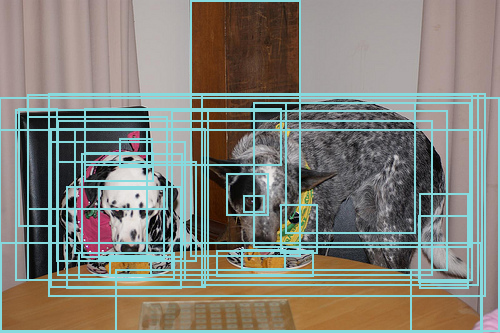
\includegraphics[width=4cm]{fig/visual_genome_dogs.png}
	\end{minipage}
	\begin{minipage}{.65\textwidth}
		\begin{tabular}{l|l}
			\hline
			Annotation	& \\	
			types		& 	\\
			\hline \hline
			Regions &  dalmatian's head; dalmatian dog\\
					& wating at a dinner table; the dog is gray\\
			Attributes & dog is gray; dalmation is eating\\
			Relationships & dog at table; dalmation IN chair; \\
							& heeler eating treat \\
							\hline
		\end{tabular}
	\end{minipage}
	\caption{Example of \vgenome. \label{fig:ex_visualgenome}}
	\end{center}
\end{figure}


\noindent
Finally, requirement~R4 is met by all discussed datasets. 

\cs{XXXXX}\\\\

\subsection{Analysis of Data wrt Our Requirements(?)}

\begin{table}[t]
	\begin{tabular}{lccc}
		\hline
		Resource & \multicolumn{3}{c}{No. categories $cat$ for which $*(cat, \text{ILSVRC})$:} \\
				& $\in$
				& superset
				& $\supset$\\
		\hline \hline
		\refcoco & 15 \\
		\refcocop & \\
		\flickr & \\
		\vgenome & \\
		\hline
	\end{tabular}
	\caption{Coverage of the categories by the $1,000$~synsets of the ILSVRC image classification challenge.  \label{tab:coverage_ilsvrc}}
\end{table}


\subsubsection{Pre-processing}
We parse referring expressions and captions with the Stanford Dependency Parser.
We extract heads/object names as follows: TODO.

\subsubsection{Level of Specificity} 
Variability of reference level in existing data sets for language \& vision?
Are resources appropriate for defining reference level?
\paragraph{WordNet?}

We hypothesize that the distance of a name's synset to the root node (entity) relates to its specificity.
We estimate this distance as the minimal path length of all synsets of a word  to the root node.

Table \ref{tab:specnames} shows the estimated levels of specificity for object names in the RefCoco data set.
We observe distances to the root between 2 and 17, meaning that there is a much more fine-grained distinction of levels than the three-way classification.

Unfortunately, the levels of specificity predicted by WordNet do not seem to reflect linguistic intuitions, here are some problematic examples from Table \ref{tab:specnames}:

\begin{itemize}
\item elephant (10) is more specific than panda (14)? horse is less specific than elephant (10)?
\end{itemize}


\begin{table}
\centering
\setlength{\tabcolsep}{4pt}
\begin{tabular}{rrl}
\toprule
 specificity &  rel.freq. &                          top 5 names \\
\midrule
          -1 &   0.071697 &      NONE,brocolli,zeb,broc,girafe \\
           2 &   0.003898 &                         thing,things \\
           3 &   0.001182 &   object,group,set,substance,objects \\
           4 &   0.140633 &           man,person,piece,head,part \\
           5 &   0.100739 &       player,glass,baby,front,corner \\
           6 &   0.208590 &              woman,girl,kid,boy,bowl \\
           7 &   0.238708 &            guy,right,chair,lady,bear \\
           8 &   0.110613 &           horse,bus,cow,pizza,batter \\
           9 &   0.097390 &         shirt,car,bike,donut,catcher \\
          10 &   0.048368 &   elephant,couch,truck,vase,suitcase \\
          11 &   0.008828 &    motorcycle,clock,mom,dad,scissors \\
          12 &   0.002822 &  oven,airplane,suv,taxi,refrigerator \\
          13 &   0.005253 &   laptop,fridge,canoe,orioles,pigeon \\
          14 &   0.000414 &  panda,freezer,penguin,rooster,rhino \\
          15 &   0.030870 &   zebra,giraffe,zebras,giraffes,deer \\
          16 &   0.000083 &       bison,mooses,orang,elks,sambar \\
          17 &   0.000143 &           ox,cattle,gnu,mustang,orca \\
\bottomrule
\end{tabular}\caption{Levels of specificity for naming choices in RefCOCO: for each level, relative frequency and 5 most frequent names are shown}
\label{tab:specnames}
\end{table}

\paragraph{No. of images in ImageNet?}

\paragraph{ImageNet and ILSVRC}


%Multiple datasets for vision \& language tasks have been built on top of COCO, such as the referring expressions datasets \refcoco and \refcocop which we will discuss below, and \textsl{COCO Captions} \cite{chen2015cococaptions}.  

\subsection{\refcoco and \refcocop \cite{Yu2016}}~\\ 
Both datasets are extensions of \referit\cite{Kazemzadeh2014}, a large-scale collection of referring expressions (RE) for natural objects in real-world images, and are built on top of the MS COCO image collection \cite{mscoco}, 
%The latter provides five captions for each of  $300k$~images, spanning $80$~of the COCO categories.  
%However, the COCO region-level (object) annotations are not linked to the captions.
a dataset of images of natural scenes of $91$~common object categories (e.g.,~\cat{dog, pizza, chair}). 
The REs were collected via crowdsourcing in a two-player game, which was designed to obtain REs uniquely referring to the target objects in an image. 
Specifically, a director and a matcher are presented with an image, and the director produces a RE for an outlined target object in the image. 
The matcher must click on the object he thinks the RE refers to. % (For more details on the datasets see \cite{Yu2016}). 
If the matcher's prediction is correct, the RE is considered valid.


\paragraph{Shortcomings}
REs in \refcoco and \refcocop were collected under the constraints that (i) all images contain at least two objects of the same category (80 COCO categories), which prompts the players to avoid the mere object category as RE, and (ii) in \refcocop the players must not use location words, urging them to refer to the appearance of objects. 
Another critical property of the data is that, (iii), not all objects in an image were annotated with REs, may it due to the frequency constraint~(i), or due to the object not being part of the 80 COCO categories. 
Finally, the $80$~COCO categories tend to be entry-level categories and are not linked to the ImageNet taxonomy. \cs{TODO: EX / ANALYSIS}

\begin{itemize}
        \item[(R1)] \textbf{Lexical choice}: is mostly met by both data sets, though it is unclear how the additional constraints in RefCoco+ impact on the naturalness of object naming
		\item[(2)] \textbf{Lexical candidates}: is not met, as we only have access to basic-level categories and cannot retrieve the  most specific category or name for each object
		\item[(3)] \textbf{Contextual informativeness}: is not met, as not all objects were annotated with REs and corresponding categories
\end{itemize}



\paragraph{Flickr30k Entities}~\\
The \flickr dataset \cite{plummer2015flickr30kentities}\footnote{Available at  \url{web.engr.illinois.edu/~bplumme2/Flickr30kEntities}}  augments Flickr30k, a dataset of 30k~images and five sentence-level captions for each of the images, with region-level annotations. 
Specifically, mentions of the same entities across the five captions of an image are linked to the bounding boxes of the objects they refer to. 
The dataset was designed to advance image description generation and phrase localization in particular (e.g.,~\cite{rohrbach2016grounding,plummer2017phrase,yeh2018unsupervised}). 


\section{Proposal}
%\label{sec:future_proposal}
%\textbf{TODO@Sina (?)}\\
%
 vision people have focussed on learning very specific categories, and have not cared about learning actual concepts/names, 
 
 language \& vision people have focussed on learning what speakers say in certain data sets, 
 we know that speakers will use object names at a medium level of specificity most of the time, 
 so it is difficult to learn the meaning of specific concepts from existing resources and to implement a model that can decide which level in the taxonomy is appropriate in context --- 
 we need a more systematic approach for collecting object naming data, 
 controlling the level of specificity (e.g. prompting speakers to come up with the most specific word they can think of)... this data might also give us insight into what basic-level and sub-level concepts are ..

%yes, will try ...

\clearpage
\bibliographystyle{splncs}
\bibliography{naming}
\end{document}
